%% ****** Start of file apstemplate.tex ****** %
\documentclass[aps,prl,reprint,groupedaddress]{revtex4-2}

% You should use BibTeX and apsrev.bst for references
% Choosing a journal automatically selects the correct APS
% BibTeX style file (bst file), so only uncomment the line
% below if necessary.
% \bibliographystyle{apsrev4-2}

\usepackage{graphicx}
\usepackage{epstopdf}
\usepackage{amsmath}
\usepackage{amsthm}
\usepackage{amsfonts}
\usepackage{subfigure}
\usepackage{hhline}
\usepackage[left=1cm,right=1cm,top=1cm,bottom=1cm]{geometry}
\usepackage[miktex]{gnuplottex}
\usepackage{xcolor}
\usepackage{amssymb}
\usepackage{amsmath}
\usepackage{color}
\usepackage{hyperref}
\usepackage[percent]{overpic}
\usepackage{tikz}
\usepackage{tikz-3dplot}
\usepackage{mathrsfs}
\usepackage{wasysym}
\usepackage{tikz-cd}  
\usepackage{caption}  % Elimina hypcap=true si está presente
\usepackage{stackengine,scalerel}
\usepackage{subcaption}
\usepackage{enumitem}
\setlist[itemize]{noitemsep}

\usepackage{caption}
\captionsetup{skip=0pt}  % Reduce el espacio entre la imagen y su caption
\raggedbottom

% so sections, subsections, etc. become numerated.
\setcounter{secnumdepth}{3}

\newenvironment{Figura}
  {\par\medskip\noindent\minipage{\linewidth}}
  {\endminipage\par\medskip}

\renewcommand{\appendixname}{Apéndice} % Change "Appendix" to "Apéndice"

\begin{document}

%Title of paper
\title{
Trabajo Integrador - Autoencoder y Clasificador con PyTorch
}

% autores
\author{Kevin Gaston Mansilla}
\email[]{kevin.mansilla@mi.unc.edu.ar}

\affiliation{}

%fecha
\date{\today}

\begin{abstract}
\end{abstract}

% insert suggested keywords - APS authors don't need to do this
%\keywords{}

%\maketitle must follow title, authors, abstract, and keywords
\maketitle

\section{Introducción}

Tomando como punto de partida la base de datos de Fashion MNIST
\footnote{https://github.com/zalandoresearch/fashion-mnist}, el objetivo de 
este trabajo es implementar un autoencoder convolucional usando PyTorch \cite{NEURIPS2019_9015} 
que es básicamente un sistema de codificación y decodificación de imágenes.

Luego de entrenarlo, realizaremos experimentos variando los 
hiperparámetros de la red para ver cómo afectan al error de reconstrucción. 
Por otro lado, implementaremos y entrenaremos un clasificador convolucional 
reutilizando el encoder del autoencoder previamente definido. 

Por último, probaremos como se comporta solo reentrenando los parámetros de la 
capa clasificadora, dejando los parámetros de la capa codificadora tal 
como vienen entrenados del autoencoder convolucional inicial.

\section{Autoencoder Convolucional}
Se puede intuir que el propósito de un autoencoder es aprender una aproximación 
de la función identidad, por medio de la reducción de la dimensionalidad,
es decir, comprimir la información de entrada en una representación de menor
dimensión.

Como se muestra en la figura \ref{fig-autoencoder} consta de dos partes, un 
encoder que comprime los datos de entrada (Compressed Representation), con el 
objetivo de obtener las características principales de dichos datos y un 
decoder que reconstruye la entrada a partir de las características encontradas 
en el encoder.
\begin{Figura}
  \centering
  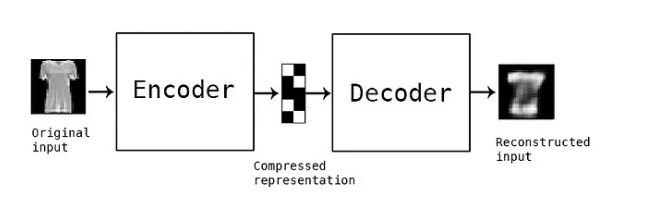
\includegraphics[width=0.90\textwidth]{figs/ejem_encoder_decoder.png}
  \captionof{figure}{Autoencoder convolucional}
  \label{fig-autoencoder}
\end{Figura}

Entrenaremos con los siguientes hiperparámetros (modelo base):
\begin{itemize}
  \item [-] $n = 64$ (número de neuronas en la capa lineal).
  \item [-] $lr = 0.001$.
  \item [-] $p = 0.2$ (probabilidad de dropout).
  \item [-] $epochs = 15$.
  \item [-] $batch\_size = 100$.
  \item [-] $loss = MSELoss$.
  \item [-] $optimizer = Adam$.
\end{itemize}

La arquitectura del encoder es la siguiente:
\begin{itemize}
  \item Una capa convolucional 2D compuesta por:
  \begin{itemize}
    \item [-] un capa $Conv2d$ de entrada de dimensiones $(1, 28, 28)$, de 
    salida $(16, 26, 26)$ y kernel $(3,3)$.
    \item [-] una capa de activación $ReLU$.
    \item [-] una capa $Dropout$.
    \item [-] una capa $MaxPool2d$, la cual mapea dimensiones $(16, 26, 26)$ a
    $(16, 13, 13)$ y kernel $(2,2)$.
  \end{itemize}
  \item Otra capa convolucional 2D compuesta por:
  \begin{itemize}
    \item [-] un capa $Conv2d$ de entrada de dimensiones $(16, 13, 13)$, de 
    salida $(32, 11, 11)$ y kernel $(3,3)$.
    \item [-] una capa de activación $ReLU$.
    \item [-] una capa $Dropout$.
    \item [-] una capa $MaxPool2d$, la cual mapea dimensiones $(32, 11, 11)$ a
    $(32, 5, 5)$ y kernel $(2,2)$.
  \end{itemize}
  \item Una capa lineal compuesta por:
  \begin{itemize}
    \item [-] una capa $Flatten$ que mapea dimensiones $(32, 5, 5)$ a $(32*5*5)$.
    \item [-] una capa $Linear$ de entrada $(32*5*5)$ y salida $n$.
    \item [-] una capa de activación $ReLU$.
    \item [-] una capa $Dropout$.
  \end{itemize}
\end{itemize}

El decoder con las siguientes capas:
\begin{itemize}
  \item Una capa lineal compuesta por:
  \begin{itemize}
    \item [-] una capa $Linear$ de entrada $n$ y salida $(32*5*5)$.
    \item [-] una capa de activación $ReLU$.
    \item [-] una capa $Dropout$.
    \item [-] una capa $Unflatten$ que mapea dimensiones $(32*5*5)$ a $(32, 5, 5)$.
  \end{itemize}
  \item Una capa convolucional 2D compuesta por:
  \begin{itemize}
    \item [-] un capa $ConvTranspose2d$ que mapea dimensiones $(32, 5, 5)$ a
    $(16, 13, 13)$, kelnel\_size $(4,4)$, stride $(2,2)$ y un 
    output\_padding de $(1,1)$.
    \item [-] una capa de activación $ReLU$.
    \item [-] una capa $Dropout$.
  \end{itemize}
  \item Otra capa convolucional 2D compuesta por:
  \begin{itemize}
    \item [-] un capa $ConvTranspose2d$ que mapea dimensione $(16, 13, 13)$ a
    $(1, 28, 28)$, kernel\_size $(4,4)$, stride $(2,2)$ y un 
    output\_padding de $(1,1)$.
    \item [-] una capa de activación $Sigmoid$.
  \end{itemize}
\end{itemize}

No le agregamos capa de $Dropout$ en la capa de salida del decoder, ya que 
este genera la salida reconstruida, que idealmente debería ser lo más similar 
posible a los datos de entrada originales, si le agregáramos esta capa 
introduciría ruido que afectaría directamente la calidad de reconstrucción.

Luego variaremos los hiperparámetros de la red para ver cómo afecta su 
desempeño. Primero variamos la probabilidad de dropout a $0.1$, luego
cambiaremos el número de neuronas en la capa lineal a $256$ con el mismo 
dropout y finalmente cambiaremos el optimizador por SGD.

\section{Clasificador Convolucional}
Una vez entrenado el autoencoder, reutilizaremos el encoder para entrenar un 
clasificador convolucional. Que tendra la siguiente arquitectura:
\begin{itemize}
  \item Una capa lineal compuesta por:
  \begin{itemize}
    \item [-] una capa $Linear$ de entrada $n$ y salida $10$.
    \item [-] una capa de activación $ReLU$.
  \end{itemize}
\end{itemize}

El clasificador será entrenado de dos formas. Primero reentrenaremos todos los
parámetros de la red y luego solo reentrenaremos la capa clasificadora, dejando 
los parámetros de la capa codificadora tal como vienen entrenados del autoencoder 
convolucional base, con el fin de comparar los resultados obtenidos.

\section{Resultados}
\subsection{Modelo base sin entrenar}

En la figura \ref{fig-model-sin-entrenar} se muestra la imagen a predecir y las
imágenes reconstruidas por el modelo sin entrenar. Se puede observar que el
modelo no es capaz de reconstruir la imagen original.

\begin{Figura}
  \centering
  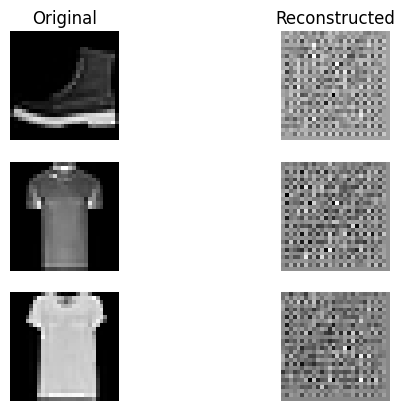
\includegraphics[width=0.4\textwidth]{figs1/modelo_sin_entrenar.png}
  \captionof{figure}{Imágenes a predecir vs imágenes reconstruidas por el modelo 
  sin entrenar}
  \label{fig-model-sin-entrenar}
\end{Figura}

\subsection{Modelo base entrenado}

Los resultados para el modelo base entrenado se presentan en la figura
\ref{fig-modelb-entrenado-perdida}. Las curvas muestran una disminución inicial 
en las funciones de pérdida a media que avanzan las épocas, sin embargo, a 
partir de la época $5$, las curvas experimentan un leve aumento seguidas de 
una leve oscilación, lo que podría ser un signo de que el modelo no va a tener 
un buen desempeño. 

Por otro lado, en la figura \ref{fig-modelb-entrenado-img} se aprecia que el modelo 
logra reconstruir la imagen original, pero con una calidad no muy buena, lo cual 
confirma lo observado en la función de pérdida.

\begin{Figura}
  \centering
  % Primera imagen
  \begin{minipage}[t]{0.58\linewidth}
    \centering
    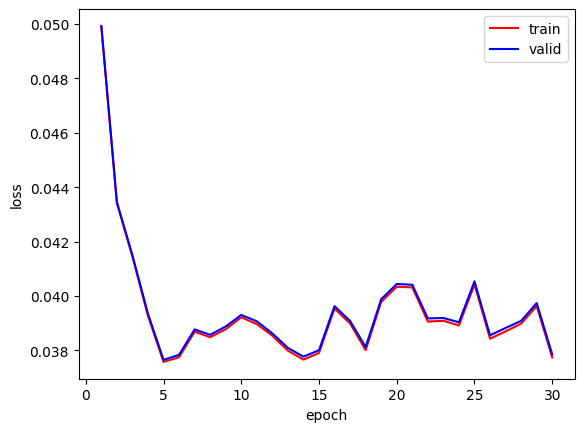
\includegraphics[width=\textwidth]{figs1/modelo_original.png}
    \captionof{figure}{Función de pérdida del modelo base entrenado}
    \label{fig-modelb-entrenado-perdida}
  \end{minipage}%
  \hfill
  % Segunda imagen
  \begin{minipage}[t]{0.41\linewidth}
    \centering
    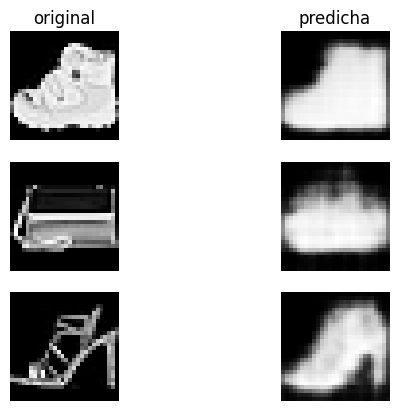
\includegraphics[width=\textwidth]{figs1/test_modelo_original.png}
    \captionof{figure}{Imágenes a predecir vs imágenes reconstruidas por el modelo
    base entrenado}
    \label{fig-modelb-entrenado-img}
  \end{minipage}
\end{Figura}

\subsection{Modelo con probabilidad de dropout 0.1, $n=64$}

En la figura \ref{fig-model-dropout01} se muestra la función de pérdida del
modelo variando solo la probabilidad de dropout a $0.1$. Identificamos un 
comportamiento similar al modelo base, pero con una oscilación no tan 
pronunciada, por lo que el cambio de este hiperparámetro no afecta 
significativamente el desempeño del modelo.

A su vez, en la figura \ref{fig-model-dropout05b} vemos que el modelo es capaz de 
captar los patrones generales de las imágenes, pero pierde información de alto 
nivel, como los bordes o los detalles más finos.

\begin{Figura}
  \centering
  % Primera imagen
  \begin{minipage}[t]{0.58\linewidth}
    \centering
    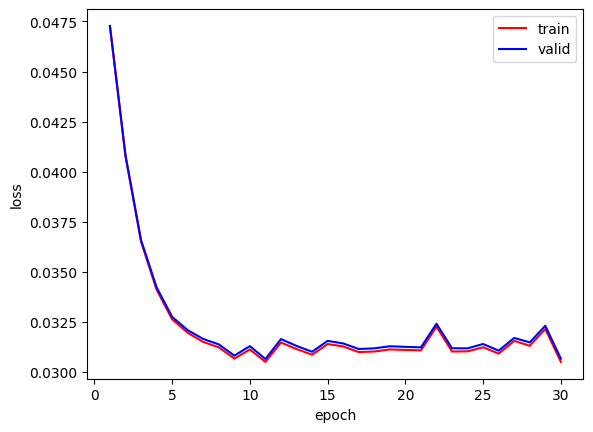
\includegraphics[width=\textwidth]{figs1/modelo_n64_dropout01.png}
    \captionof{figure}{Función de pérdida del modelo con probabilidad de dropout 0.1}
    \label{fig-model-dropout01}
  \end{minipage}%
  \hfill
  % Segunda imagen
  \begin{minipage}[t]{0.41\linewidth}
    \centering
    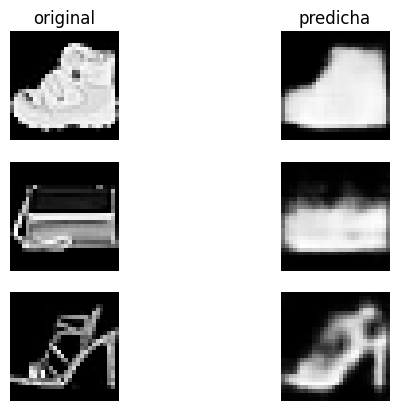
\includegraphics[width=\textwidth]{figs1/test_modelo_n64_dropout_01.png}
    \captionof{figure}{Imágenes a predecir vs imágenes reconstruidas por el modelo
    con probabilidad de dropout 0.1}
    \label{fig-model-dropout05b}
  \end{minipage}
\end{Figura}

\subsection{Modelo con probabilidad de dropout 0.1 y $n=256$}

Ahora, con un dropout de $0.1$ y $n=256$ como vemos en el gráfico 
\ref{fig-model-dropout01-256} las funciones de pérdida de ambos conjuntos 
de datos disminuyen constantemente, lo que indica que el autoencoder está logrando 
comprimir y reconstruir los datos de entrada de manera eficiente. 

La proximidad entre las curvas es casi idéntica que en los casos anteriores, 
pero al ver el eje de loss vemos que los valores son mucho mejores, lo cual
podría ser un indicio de que el modelo está aprendiendo correctamente.

En la figura \ref{fig-model-dropout01b-256} aunque no son perfectas, el modelo es 
capaz de capturar más detalles de las imágenes originales.

\begin{Figura}
  \centering
  % Primera imagen
  \begin{minipage}[t]{0.58\linewidth}
    \centering
    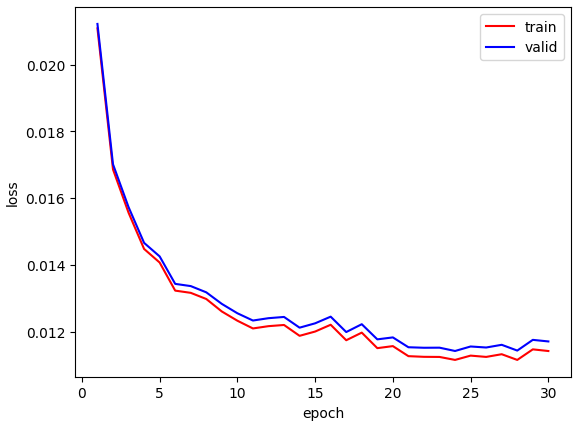
\includegraphics[width=\textwidth]{figs1/modelo_n256_dropout01.png}
    \captionof{figure}{Función de pérdida del modelo con probabilidad de dropout 
    0.1 y $n=256$}
    \label{fig-model-dropout01-256}
  \end{minipage}%
  \hfill
  % Segunda imagen
  \begin{minipage}[t]{0.41\linewidth}
    \centering
    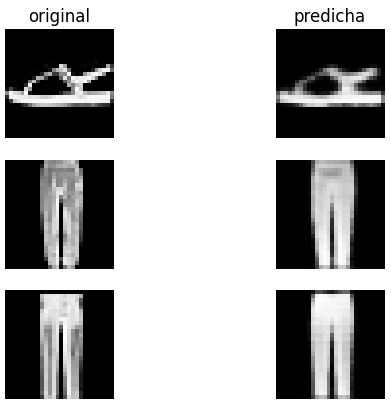
\includegraphics[width=\textwidth]{figs1/test_modelo_n256_dropout01.png}
    \captionof{figure}{Imágenea a predir vs imágenes reconstruidas por el modelo
    con probabilidad de dropout 0.1 y $n=256$}
    \label{fig-model-dropout01b-256}
  \end{minipage}
\end{Figura}

\subsection{Modelo con optimizador SGD}

Los resultados para el modelo con optimizador SGD se presentan en el gráfico 
\ref{fig-model-sgd} a simple vista vemos como las funciones de perdida de 
ambos conjuntos de datos disminuyen durante todas las épocas, esto podría
indicar que el modelo está aprendiendo correctamente. Sin embargo, al observar 
el error de esas curvas (eje loss) vemos que los valores son mucho mayores que
en los modelos anteriores, lo cual indica que el modelo no está aprendiendo
correctamente.

Confirmando lo mencionado en el párrafo previo en \ref{fig-model-sgdb}. Se puede 
observar que el modelo no es capaz de reconstruir la imagen original.

\begin{Figura}
  \centering
  % Primera imagen
  \begin{minipage}[t]{0.58\linewidth}
    \centering
    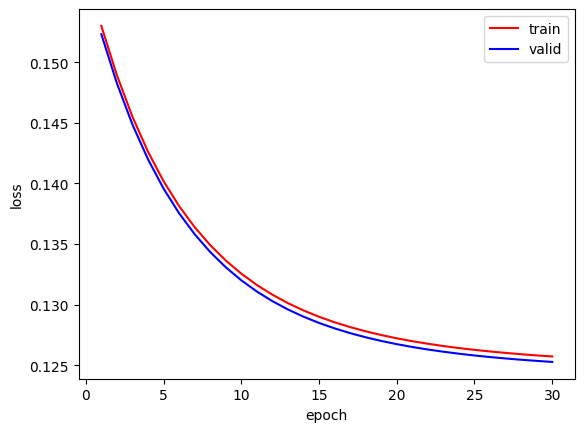
\includegraphics[width=\textwidth]{figs1/modelo_con_sdg.png}
    \captionof{figure}{Función de pérdida del modelo con optimizador SGD}
    \label{fig-model-sgd}
  \end{minipage}%
  \hfill
  % Segunda imagen
  \begin{minipage}[t]{0.41\linewidth}
    \centering
    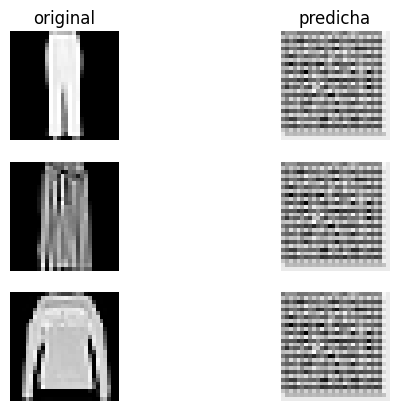
\includegraphics[width=\textwidth]{figs1/test_modelo_sdg.png}
    \captionof{figure}{Imagenea a predir vs imagenes reconstruidas por el modelo SDG}
    \label{fig-model-sgdb}
  \end{minipage}
\end{Figura}

\section{Clasificador Convolucional}

En esta sección se presentan los resultados obtenidos para el clasificador
convolucional que reutiliza el encoder del autoencoder previamente entrenado y 
en este caso se reentrenan todos los parámetros de la red por completo.

En \ref{fig-clasificador-a} se muestran las funciones de perdidas. Las curvas 
disminuyen tanto en el conjunto de entrenamiento como en el de validación a 
medida que avanzan las épocas con un error relativamente bajo, lo cual indica 
que el modelo mejora su capacidad de ajuste al avanzar las épocas.
\begin{Figura}
  \centering
  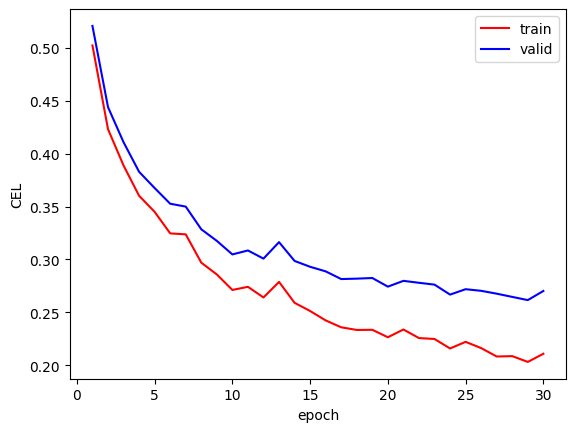
\includegraphics[width=0.60\textwidth]{figs1/modelo_con_clasificador_a.png}
  \captionof{figure}{Función de pérdida del clasificador}
  \label{fig-clasificador-a}
\end{Figura}

La precisión aumenta constantemente en ambos conjuntos de datos según se observa 
en \ref{fig-clasificador-b}, lo cual indica que el modelo es capaz de clasificar 
correctamente las imágenes de entrada.
\begin{Figura}
  \centering
  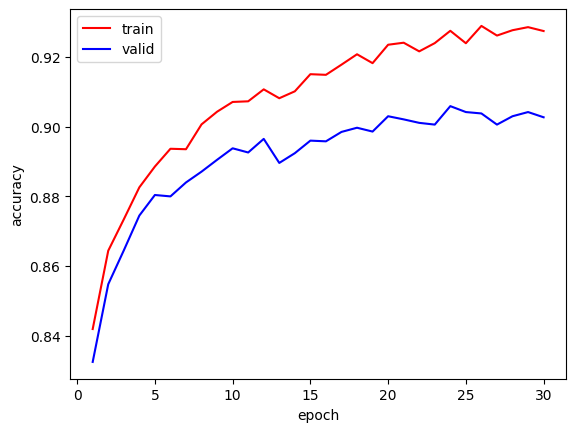
\includegraphics[width=0.60\textwidth]{figs1/modelo_con_clasificador_b.png}
  \captionof{figure}{Presición del clasificador}
  \label{fig-clasificador-b}
\end{Figura}

Y la matriz de confusión expuesta en \ref{fig-matrix}, muestra un buen desempeño 
del clasificador. Ya que en la diagonal principal presenta valores altos 
basándonos en la escala de colores de la derecha de la figura, indicando que la 
mayoría de las predicciones son correctas.

Las clases que más destacan por su desempaño con trouser, sandal, sneaker, bag 
y ankle boot. Y tiene dificultades en distinguir entre shirt y coat, por ejemplo 
tomando la fila shirt se ve que solo acierta 713 veces y 142 veces se 
equivoca prediciendo t-shirt y 60 como pullover, algo similar ocurre con coat, 
esto se debe a la similitud entre las categorías, ya que todas son prendas de 
vestir superiores.
\begin{Figura}
  \centering
  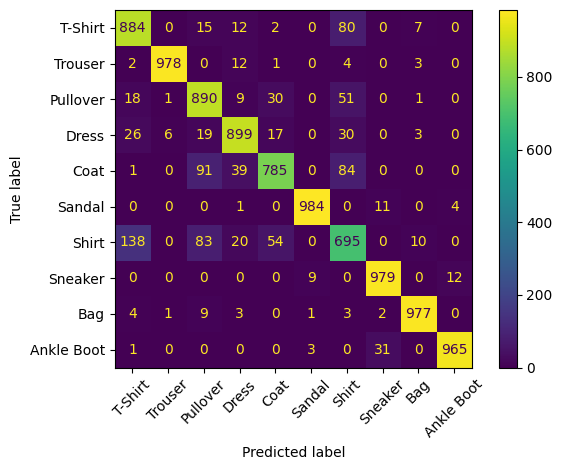
\includegraphics[width=0.80\textwidth]{figs1/matrix_confuncion_modelo_con_clasificador.png}
  \captionof{figure}{Matriz de confusión del clasificador}
  \label{fig-matrix}
\end{Figura}

\subsection{Clasificador solo entrenando la capa clasificadora}

Ahora analizamos los resultados obtenidos para el clasificador convolucional
reutilizando el encoder del autoencoder previamente entrenado en el modelo base 
y, en este caso, solo reentrenando los parámetros de la capa clasificadora. 
Es decir, que tomando como punto de partida el modelo base, solo se reentrenan 
los parámetros de la capa clasificadora y se dejan los parámetros de la capa 
codificadora tal como vienen entrenados del autoencoder convolucional.

En \ref{fig-clasificador-a-a} se muestran las funciones de pérdidas de ambos 
conjuntos de datos y presentan una disminución bastante pronunciada en ambos casos. 
El comportamiento es similar al modelo anterior, pero con un error mucho mayor.
\begin{Figura}
  \centering
  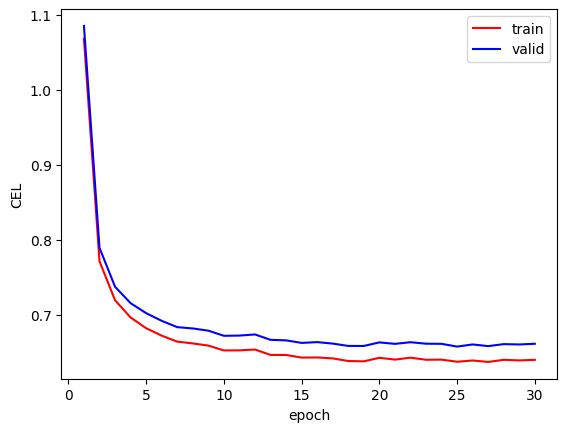
\includegraphics[width=0.60\textwidth]{figs1/modelo_original_entrenando_solo_clasificadora_a.png}
  \captionof{figure}{Función de pérdida del clasificador - solo reentrenando la capa clasificadora}
  \label{fig-clasificador-a-a}
\end{Figura}

Por otro lado, en \ref{fig-clasificador-a-b} el comportamiento de la precisión 
es diferente al modelo anterior, en este caso las curvas aumentan, pero luego se
estabilizan y comienzan a oscilar.
\begin{Figura}
  \centering
  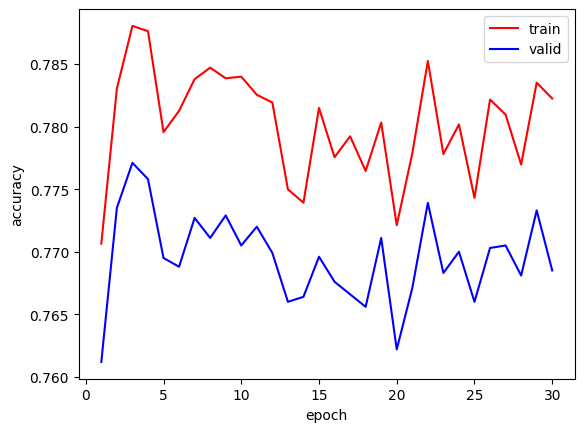
\includegraphics[width=0.60\textwidth]{figs1/modelo_original_entrenando_solo_clasificadora_b.png}
  \captionof{figure}{Presición del clasificador - solo reentrenando la capa clasificadora}
  \label{fig-clasificador-a-b}
\end{Figura}

Todo esto indica que el modelo podría llegar a tener un desempeño peor que el 
modelo anterior. A fin de comprobarlo, se muestra en \ref{fig-matrix-a} la 
matriz de confusión donde efectivamente descubrimos que el desempeño es mucho 
peor. Ya que los valores de la diagonal principal son menores en todas las 
categorías, indicando un mayor número de predicciones incorrectas.
\begin{Figura}
  \centering
  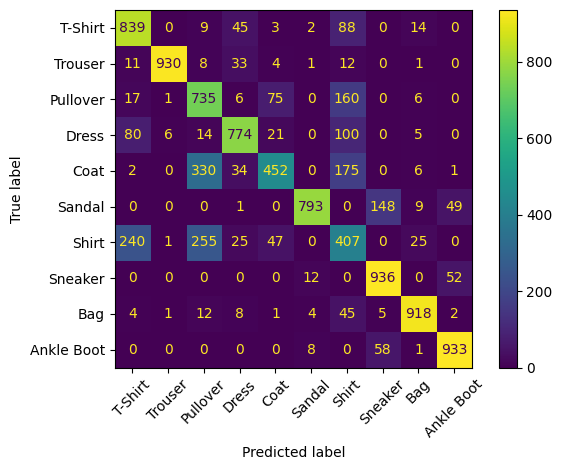
\includegraphics[width=0.80\textwidth]{figs1/matrix_confucion_modelo_original_entrenando_solo_clasificadora.png}
  \captionof{figure}{matrix de confusión - solo reentrenando la capa clasificadora}
  \label{fig-matrix-a}
\end{Figura}

Entonces concluimos que el modelo donde se reentrenan todos los parámetros de la
tiene un mejor desempeño.

\section{Conclusiones}

A lo largo de este trabajo se fueron entrenando diferentes modelos de redes
neuronales convolucionales. Inicialmente, se desarrolló un autoencoder
convolucional base sobre el cual variamos los hiperparámetros, posteriormente se 
reutilizó el encoder para entrenar un clasificador convolucional completo y, 
finalmente, se evaluaron los resultados obtenidos al reentrenar solo la capa 
clasificadora.

A medida que se incrementó la complejidad de los modelos, los resultados 
mejoraron. Sin embargo, se observó un aumento en la separación entre las curvas 
de entrenamiento y validación, lo que señala posibles signos de un desempeño 
menos robusto.

El modelo base mostró un desempeño limitado en la reconstrucción de imágenes, 
a pesar de registrar un error relativamente bajo. Al modificar la probabilidad 
de dropout a $0.1$, no se evidenciaron cambios significativos en su rendimiento. 
En contraste, al incrementar el número de neuronas en la capa lineal a $256$ 
con un dropout de $0.1$, se observó una mejora en la calidad de las imágenes 
reconstruidas. Y el modelo entrenado con el optimizador SGD presentó un desempeño 
deficiente, con un error de reconstrucción notablemente alto.

Por otro lado, el clasificador convolucional donde se reentrenaron todos los
parámetros de la red obtuvo buenos resultados, como se refleja en la matriz de 
confusión, donde la mayoría de las predicciones fueron correctas. Sin embargo, 
el clasificador que únicamente reentrenó la capa clasificadora mostró un 
rendimiento inferior al modelo anterior.

Es importante destacar que encontrar una combinación óptima de hiperparámetros 
representa un desafío considerable. Este proceso requiere una combinación de 
tiempo, recursos y experiencia para identificar los valores que maximicen el 
desempeño del modelo.

\bibliography{ref}

% Specify following sections are appendices. Use \appendix* if there
% only one appendix.

%\onecolumngrid


\end{document}
%
% ****** End of file apstemplate.tex ******